\documentclass[aspectratio=169,professionalfonts, 12pt]{beamer}
\usepackage{lmodern}
\usepackage{array}
\usepackage{multirow}
\usepackage[french,english]{babel}
\usepackage[T1]{fontenc}
\usepackage{multicol}
\usepackage{ragged2e}   %new code
\usepackage[utf8]{inputenc}
\usepackage[brazil]{varioref}
\usepackage[square,sort,comma,super,authoryear]{natbib}
\usepackage{listings,xcolor}
\usepackage{xmpmulti}
\usepackage{epsfig}
\usepackage{subcaption}
\captionsetup{compatibility=false}
\usepackage{ru,graphicx,hyperref,url} % 
\usepackage{booktabs}
\usepackage{pgfplots}
\usepackage{tikz}
\usepackage{ amsmath, amssymb, amsfonts}
\addtobeamertemplate{block begin}{}{\justifying}
\setbeamertemplate{section in toc}[sections numbered]
\AtBeginSection[]
{
  \begin{frame}[t]
  \begin{multicols}{2}
      \tableofcontents[currentsection]
    \end{multicols}
  \end{frame}

}

\date{\today}
\definecolor{blueforest}{RGB}{80,00,00}
\begin{document}
\selectlanguage{french}
\begin{frame}[plain, noframenumbering]
	\titlepage
\end{frame}
\begin{frame}[plain,t, noframenumbering]
	\frametitle{Table des matières}
    \begin{multicols}{2}
    \tableofcontents
    \end{multicols}
\end{frame}

% Section titles are shown in at the top of the slides with the current section 
% highlighted. Note that the number of sections determines the size of the top 
% bar, and hence the university name and logo. If you do not add any sections 
% they will not be visible.
\section{INTRODUCTION}

\subsection{Contexte}

\begin{frame}
  \frametitle{Contexte}
  \justifying 
  \begin{minipage}{\textwidth}
  \begin{block}{}
  Les systèmes informatisés conservent généralement des données détaillées des interactions utilisateur-système, plus précisément des interactions système-apprenant dans les systèmes éducatifs et les systèmes de tutorat intelligent (ITS). Ces données détaillées qui sont dans une grande base de données offrent des opportunités pour étudier ces données récolter.  
  \end{block}
  \only<1->
  \end{minipage}
\end{frame}

% \begin{frame}
%   \frametitle{Contexte(suite)}
%   \justifying 
%   \begin{minipage}{\textwidth}
%   \begin{itemize}
%     \item 1
%     \item 2
%     \item 3
%     \item 4
%   \end{itemize}
%   \end{minipage}
% \end{frame}

\subsection{Problématique}
\begin{frame}
  \frametitle{Problématique}
  \justifying
  \begin{alertblock}{Problèmes}
  Cependant les données ne sont jamais aussi complètes et sans équivoque qu’elles garantissent la certitude. \\
  Aussi, dans les systèmes éducatifs, beaucoup d’aptitudes ont une forte relation causale dans laquelle une aptitude doit être présentée avant une autre.
\end{alertblock}
\end{frame}

\subsection{Objectif}

\begin{frame}
  \frametitle{Objectif}
  \begin{block}{L'objectif principal}
    Analyse et évaluation du jeu de données en faisant un ajustement bayésien des réponses aux items avant de décider si oui ou non le jeu de données valle le coup d’être utilisé.\\
    Après la validation du jeu de données, les items sont regroupés en composante de connaissance en utilisant une approche basée sur la similarité qui utilise une matrice de similarité calculée selon quatre catégories : réponse correcte et incorrecte avec aide et sans aide.
  \end{block}     
\end{frame}

\section{APERÇU SUR L'\'ETAT DE L'ART}
\subsection{Educational data minig}

\begin{frame}
  \frametitle{Educational data minig}
  \justifying 
  \begin{minipage}{\textwidth}
  \begin{block}{}
    L’exploration de données est un processus itératif et interactif visant à découvrir des modèles de données efficaces, nouveaux, utiles et compréhensibles dans de grandes bases de données. Appliquer dans l’éducation, les données proviennent du milieu éducatif et le but est de comprendre le comportement des apprenants et l’environnement de leur apprentissage.  
  \end{block}
  \end{minipage}
\end{frame}

\begin{frame}
  \frametitle{Educational data minig}
  \justifying 
  \begin{minipage}{\textwidth}
  \begin{figure}[H]
      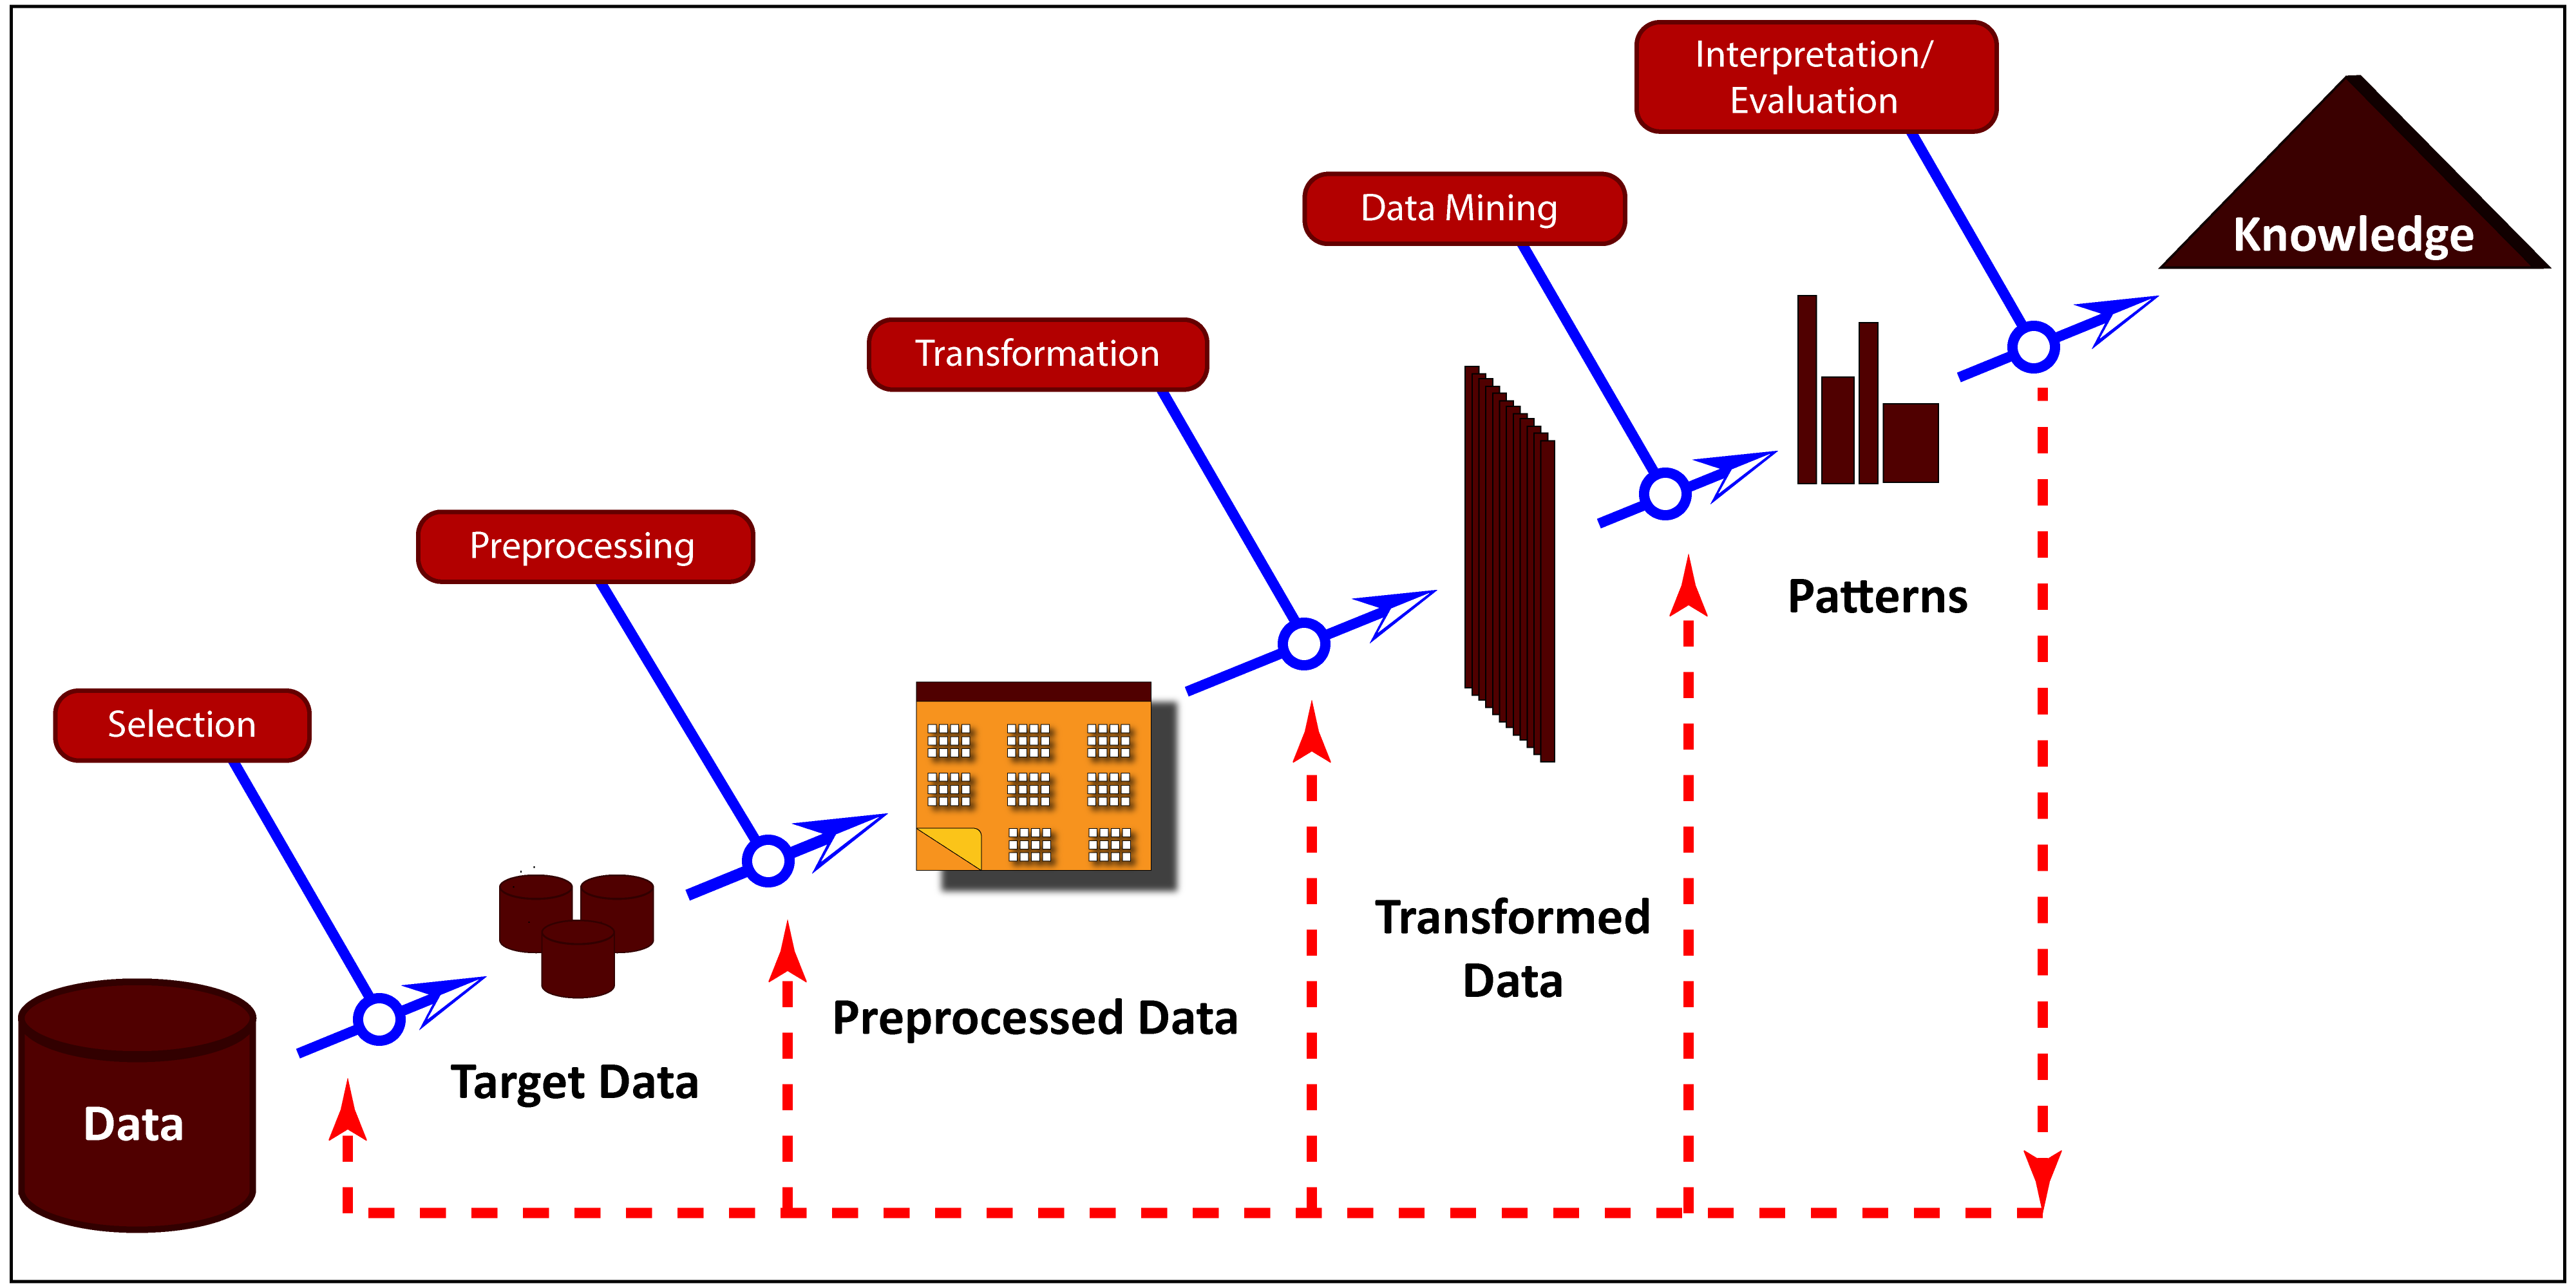
\includegraphics[height=6cm]{images/etat_art/extract_data_steps.png}
  \end{figure}
  \end{minipage}
\end{frame}


\subsection{Modèle de l’apprenant}

\begin{frame}
  \frametitle{Modèle de l’apprenant}
  \justifying 
  \begin{minipage}{\textwidth}
  \begin{block}{Définition}
    Le modèle de l’apprenant est une structure de données qui reflète l’état des connaissances supposées de l’apprenant sur un domaine cible.
  \end{block}
    \only<1->
  \end{minipage} 
  \begin{minipage}{\textwidth}
  \onslide<2->
  \begin{block}{}
    Quelque catégorie du modèle de l’apprenant :
    \begin{itemize}
      \item Modèle cognitif,
      \item Modèle d’inférence,
      \item Modèle émotionnel.
    \end{itemize}
  \end{block}
  \end{minipage}
\end{frame}

\begin{frame}
  \frametitle{Modèle de l’apprenant}
  \justifying 
  \begin{minipage}{\textwidth}
  \begin{block}{L’approche du modèle cognitif}
    La modélisation cognitive est utilisé pour simuler ou prédire le comportement humain ou les performances sur des tâches similaires à celles modélisées et améliorer l'interaction homme-machine.  \end{block}
  \only<1->
  \end{minipage} 
  \begin{minipage}{\textwidth}
    \begin{figure}[H]
      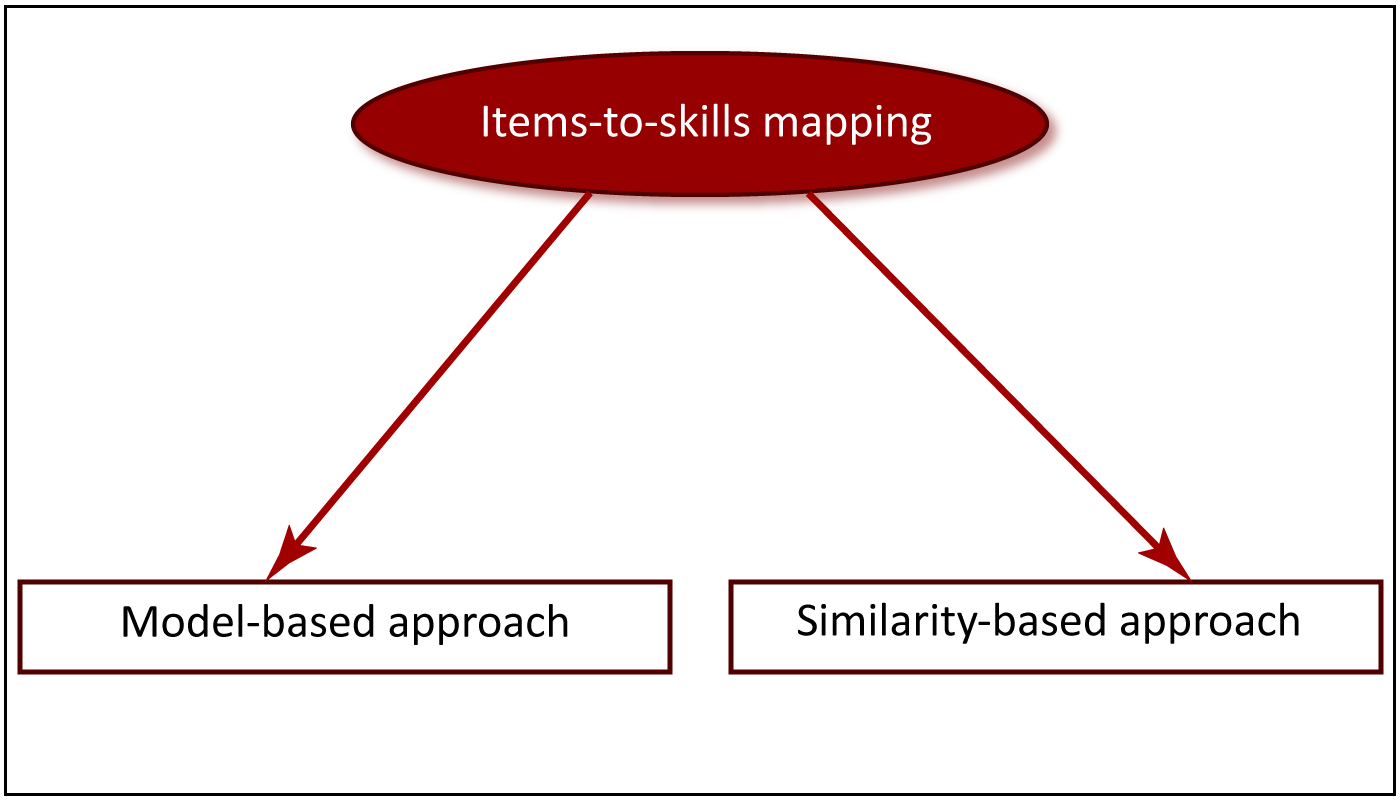
\includegraphics[ height=3.6cm]{images/etat_art/Items_mapping_structure.png}
    \end{figure}
  \end{minipage}
\end{frame}

\begin{frame}
  \frametitle{Modèle de l’apprenant}
  \justifying 
  \begin{minipage}{\textwidth}
  \begin{block}{L’approche du modèle d’inférence}
    Cette approche est une sorte de moteur d’inférence qui fonctionne pour ajuster le modèle de l’apprenant. Il contient des règles qui lui permettent de raisonner sur le modèle cognitif et sur le modèle psychologique pour inférer de nouvelles connaissances dans le modèle de l’apprenant.  
  \end{block}
  \end{minipage} 
\end{frame}

\subsection{Inférence bayésienne}

\begin{frame}
  \frametitle{Inférence bayésienne}
  \justifying 
  \begin{minipage}{\textwidth}
  \begin{block}{Définition}
    L’inférence bayésienne est une méthode d’apprentissage des valeurs des paramètres dans les modèles statistiques à partir de données. 
  \end{block}
  \end{minipage} 
\end{frame}


\begin{frame}
  \frametitle{Inférence bayésienne}
  \begin{minipage}{0.6\textwidth}
  \begin{block}{Probabilité conditionnelle}
    La probabilité conditionnelle est la probabilité d'un événement sachant qu'un autre événement a eu lieu.\\
    Soit \(\displaystyle A \)  et \(\displaystyle B \) deux évènements avec \(\displaystyle P(A) \neq 0 \).
    \begin{equation}
      P(B|A) = \frac{P(A\cap B)}{P(A)}
      \label{conditionnelle_probability}
    \end{equation}
  \end{block}
  \end{minipage}
  \begin{minipage}{2cm}
  
  \end{minipage}
  \begin{minipage}{0.3\textwidth}
    \begin{figure}[t]
    \begin{center}
      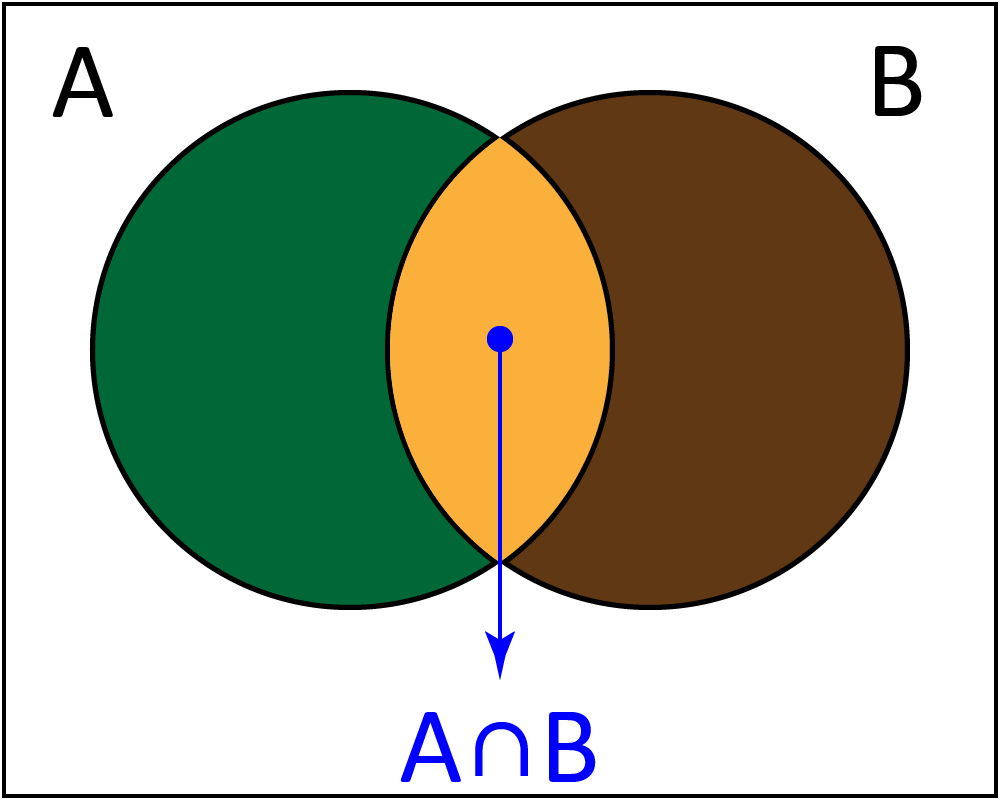
\includegraphics[width=\textwidth]{images/etat_art/conditional_b.png}
    \end{center}
    \end{figure} 
  \end{minipage}	
\end{frame}

\begin{frame}
  \frametitle{Inférence bayésienne}
  \justifying 
  \begin{minipage}{\textwidth}
  \begin{block}{Théorème de bayes}
    Le théorème de Bayes , du nom du mathématicien britannique du XVIIIe siècle Thomas Bayes est definit par l'équation suivante:   
    \begin{equation}
      Pr(B|A) = \frac{P(A\cap B)}{P(A)} = \frac{Pr(A|B)*Pr(B)}{Pr(A)}
      \label{theoreme_bayes}
    \end{equation} 
    \begin{equation}
      Pr(hypothesis|data) = \frac{Pr(data|hypothesis)*Pr(hypothesis)}{Pr(data)}
      \label{theoreme_bayes2}
    \end{equation}
  \end{block}
  \end{minipage} 
\end{frame}

%L’approche Bayésienne

\begin{frame}
  \frametitle{Inférence bayésienne}
  \justifying 
  \begin{minipage}{\textwidth}
  \begin{block}{L’approche Bayésienne}
    L'inférence bayésienne utilise la règle de bayes lorsqu’on interprète les variables de la règle de Bayes en tant que paramètres \(\displaystyle \theta \) d'un modèle et de données observées \(\displaystyle data \) : 
  \end{block}
  \end{minipage}
  \begin{minipage}{\textwidth}
    \centering
  \onslide<2->    
    \begin{equation}
      \color{red} Pr(\theta|data) = \color{blue} \frac{Pr(data|\theta)\color{black} * \color{green}Pr(\theta)}{ \color{blueforest} Pr(data) =  \int_{}^{}  \,L(data|\theta)Pr(\theta)d\theta }
      \label{theoreme_bayes3}
    \end{equation}
  \end{minipage}
\end{frame}

\subsection{La théorie de la réponse à items}

\begin{frame}
  \frametitle{La théorie de la réponse à items}
  \framesubtitle{Quelque définitions}
  \justifying 
  \begin{minipage}{\textwidth}
  \begin{block}{}
    La théorie de la réponse à l'item fait référence aux modèles mathématiques qui tentent d'expliquer la relation entre les traits latents et leurs manifestations.
  \end{block}


  \end{minipage} 
\end{frame}

\begin{frame}
  \frametitle{La théorie de la réponse à items}
  \justifying 
  \begin{minipage}{\textwidth}
  \begin{figure}[H]
      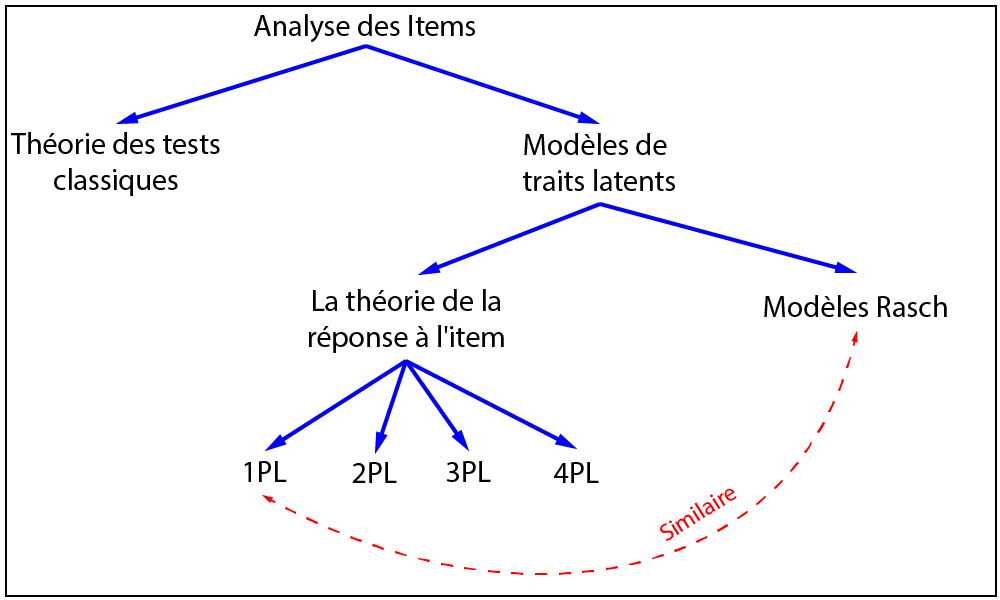
\includegraphics[height=6cm]{images/etat_art/items_analysis.png}
  \end{figure}
  \end{minipage}
\end{frame}


\begin{frame}
  \frametitle{La théorie de la réponse à items}
  \justifying 
  \begin{minipage}{\textwidth}
  \begin{block}{Théorie des tests classiques}
  \end{block}  
  \end{minipage} 
\end{frame}

\begin{frame}
  \frametitle{La théorie de la réponse à items}
  \justifying 
  \begin{minipage}{\textwidth}
  \begin{block}{Théorie des tests classiques vs modèles de traits latents}
  \end{block}  
  \end{minipage} 
\end{frame}

\begin{frame}
  \frametitle{La théorie de la réponse à items}
  \justifying 
  \begin{minipage}{\textwidth}
  \begin{block}{Modèles de traits latents}
  \end{block}  
  \end{minipage} 
\end{frame}

\begin{frame}
  \frametitle{La théorie de la réponse à items}
  \justifying 
  \begin{minipage}{\textwidth}
  \begin{block}{Avantages de l'IRT}
    \begin{itemize}
      \item	Fournit plus d'informations que la théorie des tests classique (CTT).
      \begin{itemize}
        \item Les statistiques des tests classiques dépendent de l'ensemble des éléments et de l'échantillon examinés.
        \item	Modélisation IRT indépendante de l'échantillon examiné.
      \end{itemize}
      \item Utilisé pour estimer les paramètres des éléments (par exemple, la difficulté et la discrimination) et...
      \item Les vrais scores de la personne sur le trait latent.
    \end{itemize}
  \end{block}  
  \end{minipage} 
\end{frame}

\section{CONTRIBUTIONS}

\subsection{Approche proposée}

\subsection{Résultats}

\subsection{Comparaison}

\section{CONCLUSION G\'EN\'ERALE}

\end{document}
